\documentclass[conference]{IEEEtran}
\IEEEoverridecommandlockouts
\usepackage{cite}
\usepackage{amsmath,amssymb,amsfonts}
\usepackage{algorithmic}
\usepackage{graphicx}
\usepackage{textcomp}
\usepackage{xcolor}
\usepackage{svg}
\usepackage[utf8]{inputenc}
\usepackage[spanish]{babel}
\addto\captionsspanish{\renewcommand{\tablename}{Tabla}}
\usepackage{listings}
\usepackage{caption}
\captionsetup[table]{skip=10pt}

\renewcommand{\lstlistingname}{Código}

\lstset{
  language=Python,
  basicstyle=\ttfamily\small,
  frame=single,
  breaklines=true,
  keywordstyle=\color{blue},
  commentstyle=\color{gray},
  stringstyle=\color{teal},
  numbers=left,
  numberstyle=\tiny,
  captionpos=b
}

\title{Laboratorio 04: Clasificadores de ensamble\\
\vspace{0.5em} \huge \textbf{Asignatura}: \textit{Machine Learning} (2026-01)\\
\vspace{0.5em} \large \textbf{Profesor}: Dr. Juan Bekios Calfa}

\author{
\IEEEauthorblockN{1\textsuperscript{st} Pablo López}
\IEEEauthorblockA{\textit{Escuela de Ingeniería} \\
\textit{Universidad Católica del Norte}\\
Ingeniería Civil en Computación e Informática\\
\texttt{pablo.lopez01@alumnos.ucn.cl}}
\and
\IEEEauthorblockN{2\textsuperscript{nd} Ignacio García}
\IEEEauthorblockA{\textit{Escuela de Ingeniería} \\
\textit{Universidad Católica del Norte}\\
Ingeniería Civil en Computación e Informática\\
\texttt{ignacio.garcia02@alumnos.ucn.cl}}
\and
\IEEEauthorblockN{3\textsuperscript{rd} Eros Cortés}
\IEEEauthorblockA{\textit{Escuela de Ingeniería} \\
\textit{Universidad Católica del Norte}\\
Ingeniería Civil en Computación e Informática\\
\texttt{eros.cortes@alumnos.ucn.cl}}
}

\begin{document}

\maketitle

\begin{abstract}
Este informe presenta el desarrollo del Laboratorio 04 de Machine Learning, centrado en la comparación de clasificadores de ensamble aplicados a un dataset SPSS con 15 atributos y seis objetivos de clasificación. Se implementaron y evaluaron Bagging, AdaBoost, Stacking y Gradient Boosting usando validación cruzada anidada, con \textit{GridSearchCV} y \textit{RandomizedSearchCV} para la selección de hiperparámetros. La métrica principal fue F1 macro, debido al desbalance observado en las clases. Los mejores resultados variaron según el objetivo: Stacking obtuvo el mayor F1 macro en GDS, Gradient Boosting destacó en GDS\_R1 y GDS\_R2, AdaBoost en GDS\_R3, y Bagging en GDS\_R4 y GDS\_R5. Los resultados muestran que no existe un ensamble dominante para todos los objetivos y que la evaluación debe considerar tanto desempeño promedio como estabilidad y soporte de clases.
\end{abstract}

\section{Introducción}
El laboratorio aborda un problema de clasificación supervisada sobre un conjunto de datos originalmente almacenado en formato SPSS. El dataset contiene 1119 registros, 15 atributos de entrada y seis objetivos de clasificación: GDS, GDS\_R1, GDS\_R2, GDS\_R3, GDS\_R4 y GDS\_R5. Cada objetivo representa una agrupación distinta de clases, por lo que el mismo conjunto de atributos se evalúa bajo escenarios de clasificación con distinta dificultad y distinto nivel de desbalance.

La motivación principal es comparar estrategias de ensamble bajo un protocolo experimental reproducible. Los ensambles combinan varios modelos individuales para mejorar la capacidad predictiva, reducir varianza o corregir errores secuencialmente. En este laboratorio se evalúan cuatro enfoques: Bagging, AdaBoost, Stacking y Gradient Boosting. La comparación se realiza con validación cruzada anidada para separar la selección de hiperparámetros de la estimación final del rendimiento.

El objetivo general es analizar el comportamiento de clasificadores de ensamble sobre los seis objetivos del dataset. Como objetivos específicos, se busca configurar hiperparámetros desde un archivo YAML, ejecutar búsquedas exhaustivas y aleatorias, reportar métricas macro adecuadas para clases desbalanceadas, revisar matrices de confusión y discutir las limitaciones metodológicas derivadas del bajo soporte en algunas clases.

El desarrollo se implementó en Python utilizando \textit{scikit-learn}, \textit{pandas}, \textit{numpy}, \textit{scipy}, \textit{pyreadstat} y \textit{PyYAML}. La ejecución se organizó mediante módulos separados para carga de datos, definición de modelos, evaluación y generación de reportes.

\section{Marco Teórico}
Un clasificador de ensamble combina varios modelos base para producir una predicción final. La hipótesis general es que una combinación de clasificadores puede obtener un rendimiento más robusto que un único modelo individual, especialmente cuando los errores de los modelos base no son idénticos.

\textbf{Bagging} entrena múltiples clasificadores sobre muestras bootstrap del conjunto de entrenamiento. En este laboratorio se usa \textit{BaggingClassifier} con árboles de decisión como estimadores base. Su principal ventaja es la reducción de varianza, ya que promedia o vota entre modelos entrenados sobre subconjuntos distintos de datos.

\textbf{AdaBoost} construye un ensamble secuencial de clasificadores débiles. Después de cada iteración, aumenta el peso de los ejemplos mal clasificados, obligando al siguiente estimador a enfocarse en casos difíciles. En este laboratorio se emplean árboles de decisión poco profundos como clasificadores base.

\textbf{Stacking} combina modelos base mediante un meta-clasificador. Los modelos base generan predicciones o probabilidades que se usan como nuevas características para entrenar un clasificador final. La implementación usada incluye árbol de decisión, K-NN escalado y regresión logística escalada, con regresión logística como meta-modelo.

\textbf{Gradient Boosting} también es un método secuencial, pero cada nuevo árbol intenta corregir los errores residuales del ensamble acumulado. Los hiperparámetros relevantes incluyen número de estimadores, tasa de aprendizaje, profundidad de los árboles y proporción de muestras usadas en cada etapa.

La métrica principal fue F1 macro. Esta métrica calcula el F1 de cada clase y luego promedia todos los valores, asignando el mismo peso a cada clase. Esto es apropiado cuando existe desbalance, ya que evita que una clase mayoritaria domine la evaluación. También se reportaron \textit{balanced accuracy}, precisión macro, recall macro, estabilidad e ICN. La validación cruzada anidada se utilizó para evitar una estimación optimista: el ciclo interno selecciona hiperparámetros y el ciclo externo estima el rendimiento final.

\section{Metodología}
El dataset contiene 1119 observaciones y 15 atributos de entrada. Los atributos corresponden a variables codificadas como valores numéricos, y los objetivos corresponden a distintas agrupaciones de clases. La Tabla~\ref{tab:distribucion} resume el soporte por objetivo.

\begin{table}[!h]
\centering
\begin{tabular}{|c|c|c|}
\hline
\textbf{Objetivo} & \textbf{Clases y soporte} & \textbf{$n_{min}$} \\
\hline
GDS & 1:149, 2:500, 3:298, 4:108, 5:42, 6:20, 7:2 & 2 \\
GDS\_R1 & 1:947, 2:150, 3:22 & 22 \\
GDS\_R2 & 1:649, 2:298, 3:172 & 172 \\
GDS\_R3 & 1:947, 3:172 & 172 \\
GDS\_R4 & 1:149, 2:906, 3:64 & 64 \\
GDS\_R5 & 1:149, 2:798, 3:172 & 149 \\
\hline
\end{tabular}
\caption{Distribución de clases para los seis objetivos.}
\label{tab:distribucion}
\end{table}

La carga de datos se realizó desde el archivo \texttt{datasets/15 atributos R0-R5.sav}. Se seleccionaron las 15 columnas de atributos definidas en el código y se transformaron a tipo flotante. Cada objetivo se convirtió a entero para ser usado por los clasificadores. No se aplicó balanceo artificial ni modificación del dataset, ya que el foco del laboratorio fue comparar ensambles bajo un protocolo común.

Los modelos se organizaron en \texttt{src/models.py}. La evaluación se implementó en \texttt{src/evaluation.py}, donde se calcula el número de folds externos como:

\begin{equation}
k_{outer} = \min(5, n_{min})
\end{equation}

Esta regla evita solicitar más particiones estratificadas que ejemplos disponibles en la clase minoritaria. En el caso de GDS, el soporte mínimo es 2; por tanto, el ciclo externo queda limitado a dos folds. Además, en algunos entrenamientos externos una clase queda con solo un ejemplo, por lo que el ciclo interno utiliza \textit{KFold} no estratificado y registra una advertencia metodológica.

Los hiperparámetros se configuraron en \texttt{config/paths.yaml}. Se ejecutaron dos experimentos: \texttt{grid\_all}, basado en \textit{GridSearchCV}, y \texttt{random\_all}, basado en \textit{RandomizedSearchCV}. Ambos usaron F1 macro como métrica de selección. Las semillas de aleatoriedad se centralizaron para controlar particiones, modelos y búsquedas aleatorias.

\section{Resultados}
La Tabla~\ref{tab:mejores} muestra el mejor resultado por objetivo considerando todos los modelos y ambos tipos de búsqueda. Los valores corresponden al promedio de F1 macro sobre los folds externos.

\begin{table}[!h]
\centering
\begin{tabular}{|c|c|c|c|}
\hline
\textbf{Objetivo} & \textbf{Mejor modelo} & \textbf{Búsqueda} & \textbf{F1 macro} \\
\hline
GDS & Stacking & grid & 0.362 \\
GDS\_R1 & Gradient Boosting & grid & 0.729 \\
GDS\_R2 & Gradient Boosting & grid & 0.669 \\
GDS\_R3 & AdaBoost & random & 0.800 \\
GDS\_R4 & Bagging & grid & 0.615 \\
GDS\_R5 & Bagging & random & 0.577 \\
\hline
\end{tabular}
\caption{Mejor F1 macro por objetivo.}
\label{tab:mejores}
\end{table}

\begin{figure}[!h]
\centering
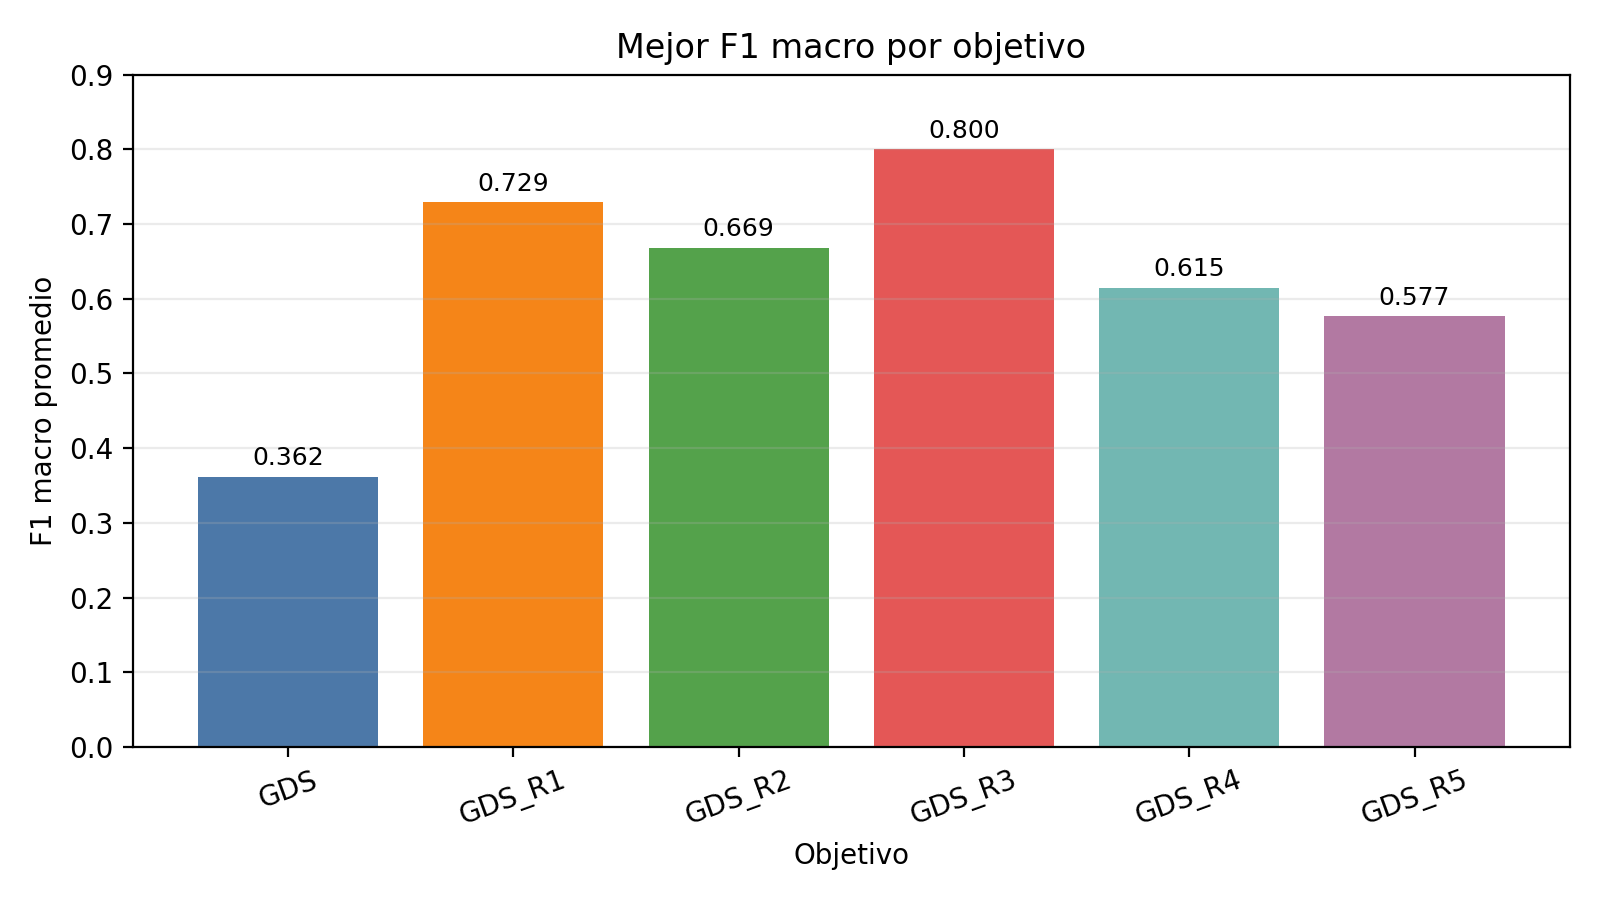
\includegraphics[width=0.48\textwidth]{images/f1_macro_final.png}
\caption{Mejor F1 macro promedio por objetivo.}
\label{fig:f1macro}
\end{figure}

La Tabla~\ref{tab:metricas} resume métricas adicionales para los mejores modelos. Se observa que los objetivos GDS\_R3 y GDS\_R1 alcanzan los mayores F1 macro, mientras que GDS es el caso más débil debido al fuerte desbalance y al soporte mínimo de solo dos ejemplos en una clase.

\begin{table*}[!t]
\centering
\begin{tabular}{|c|c|c|c|c|c|c|}
\hline
\textbf{Objetivo} & \textbf{Modelo} & \textbf{F1 macro} & \textbf{Bal. Acc.} & \textbf{Prec. macro} & \textbf{Recall macro} & \textbf{ICN} \\
\hline
GDS & Stacking & 0.362 & 0.470 & 0.363 & 0.470 & 0.907 \\
GDS\_R1 & Gradient Boosting & 0.729 & 0.718 & 0.762 & 0.718 & 0.658 \\
GDS\_R2 & Gradient Boosting & 0.669 & 0.649 & 0.703 & 0.649 & 0.552 \\
GDS\_R3 & AdaBoost & 0.800 & 0.795 & 0.808 & 0.795 & 0.692 \\
GDS\_R4 & Bagging & 0.615 & 0.649 & 0.621 & 0.649 & 0.854 \\
GDS\_R5 & Bagging & 0.577 & 0.629 & 0.568 & 0.629 & 0.853 \\
\hline
\end{tabular}
\caption{Métricas de los mejores modelos por objetivo.}
\label{tab:metricas}
\end{table*}

Para analizar errores específicos se revisaron matrices de confusión. En GDS\_R3, el mejor modelo fue AdaBoost con búsqueda aleatoria. La matriz de confusión agregada se muestra en la Tabla~\ref{tab:cmr3}. El modelo clasificó correctamente 894 ejemplos de la clase 1 y 111 ejemplos de la clase 3. El F1 por clase fue 0.940 para la clase 1 y 0.661 para la clase 3, evidenciando el efecto del desbalance.

\begin{table}[!h]
\centering
\begin{tabular}{|c|c|c|}
\hline
\textbf{Real / Pred.} & \textbf{1} & \textbf{3} \\
\hline
1 & 894 & 53 \\
3 & 61 & 111 \\
\hline
\end{tabular}
\caption{Matriz de confusión para GDS\_R3 con AdaBoost random.}
\label{tab:cmr3}
\end{table}

En GDS\_R5, el mejor resultado fue obtenido por Bagging con búsqueda aleatoria. La Tabla~\ref{tab:cmr5} muestra que la clase 2, mayoritaria, concentra la mayor cantidad de aciertos, mientras que la clase 1 tiene menor F1 por clase. Los F1 por clase fueron 0.365, 0.715 y 0.650 para las clases 1, 2 y 3, respectivamente.

\begin{table}[!h]
\centering
\begin{tabular}{|c|c|c|c|}
\hline
\textbf{Real / Pred.} & \textbf{1} & \textbf{2} & \textbf{3} \\
\hline
1 & 82 & 65 & 2 \\
2 & 215 & 508 & 75 \\
3 & 3 & 49 & 120 \\
\hline
\end{tabular}
\caption{Matriz de confusión para GDS\_R5 con Bagging random.}
\label{tab:cmr5}
\end{table}

\section{Discusión}
Los resultados muestran que no existe un único modelo ganador para todos los objetivos. Stacking fue el mejor en GDS, Gradient Boosting obtuvo los mejores resultados en GDS\_R1 y GDS\_R2, AdaBoost destacó en GDS\_R3, y Bagging fue superior en GDS\_R4 y GDS\_R5. Esto confirma que el comportamiento de los ensambles depende de la estructura del objetivo, el nivel de desbalance y la forma en que se agrupan las clases.

El caso GDS debe interpretarse con especial cautela. Aunque Stacking obtuvo el mayor F1 macro para este objetivo, la clase menos frecuente tiene solo dos ejemplos. Esto limita la validación externa a dos folds y obliga al ciclo interno a usar \textit{KFold} no estratificado cuando una clase queda con un solo ejemplo en entrenamiento. Por tanto, el valor de F1 macro en GDS es menos estable que en los demás objetivos.

En GDS\_R3 se obtuvo el mejor F1 macro global, superando levemente 0.80. Sin embargo, las métricas por clase muestran que el rendimiento no es homogéneo: la clase mayoritaria alcanza F1 de 0.940, mientras que la clase minoritaria alcanza 0.661. Esto evidencia la importancia de usar F1 macro y no solo exactitud global. En GDS\_R5, Bagging logra buen comportamiento relativo, pero la matriz de confusión muestra confusión importante entre las clases 1 y 2.

La comparación entre \textit{GridSearchCV} y \textit{RandomizedSearchCV} también resulta relevante. Algunos objetivos favorecieron la búsqueda exhaustiva y otros la búsqueda aleatoria. RandomizedSearchCV permitió explorar rangos más amplios sin evaluar todas las combinaciones posibles, mientras que GridSearchCV fue útil en espacios pequeños y controlados. La configuración desde YAML facilitó modificar los hiperparámetros sin alterar la lógica del código.

\section{Conclusiones}
El laboratorio permitió comparar cuatro estrategias de ensamble bajo un protocolo reproducible y defendible. La principal conclusión es que no existe un ganador universal: cada objetivo favoreció un modelo distinto. Esto refuerza la necesidad de evaluar múltiples modelos y no seleccionar una técnica solo por su desempeño en un único objetivo.

El uso de F1 macro fue adecuado debido al desbalance de clases. Métricas como accuracy habrían sido menos informativas, especialmente en objetivos donde una clase concentra gran parte de los registros. La validación cruzada anidada permitió separar selección de hiperparámetros y estimación del desempeño, reduciendo el riesgo de optimismo experimental.

La principal limitación fue el bajo soporte de algunas clases, especialmente en GDS. Esta condición no invalida el experimento, pero obliga a interpretar sus resultados con cautela. Como trabajo futuro se podría comparar el efecto de estrategias de balanceo, siempre que el objetivo metodológico lo permita, o explorar criterios de selección que penalicen de forma más explícita la inestabilidad entre folds.

\section{Código y Reproducibilidad}
El proyecto se organizó de forma modular. El archivo \texttt{main.py} orquesta la ejecución completa. El módulo \texttt{src/data\_loader.py} carga el archivo SPSS y prepara matrices de atributos y objetivos. El módulo \texttt{src/models.py} define los clasificadores de ensamble. El módulo \texttt{src/evaluation.py} implementa validación cruzada anidada, búsquedas de hiperparámetros y cálculo de métricas. Finalmente, \texttt{src/reports.py} genera archivos CSV, JSON, LaTeX, PDF, matrices de confusión y métricas por clase.

La configuración experimental se encuentra en \texttt{config/paths.yaml}. En este archivo se definen rutas, objetivos, experimentos, semillas, métrica de selección, número máximo de folds e hiperparámetros para búsqueda grid y random. Esta separación mejora la reproducibilidad porque permite modificar el experimento sin alterar el código fuente.

La ejecución completa se realiza con el comando mostrado en el Código~\ref{lst:ejecucion}. También se pueden ejecutar subconjuntos de objetivos, modelos o experimentos mediante argumentos de línea de comandos.

\begin{lstlisting}[caption={Ejecución completa del laboratorio}, label={lst:ejecucion}]
python main.py
\end{lstlisting}

Los resultados principales se almacenaron en \texttt{outputs/tables/resumen\_resultados.csv}. Las advertencias metodológicas quedaron en \texttt{outputs/advertencias.txt}; la advertencia principal corresponde a GDS por soporte insuficiente en el ciclo interno. Además, algunas combinaciones aleatorias de AdaBoost fueron descartadas por \textit{scikit-learn} al producir ajustes no válidos, quedando registradas con puntaje no finito. La ejecución finalizó correctamente y generó tablas, matrices de confusión y métricas por clase.

\appendices

\section{Anexos}
Los archivos generados por el laboratorio incluyen:

\begin{itemize}
  \item \texttt{outputs/tables/resumen\_resultados.csv}: resumen tabular de métricas por modelo, objetivo y experimento.
  \item \texttt{outputs/tables/resultados\_detallados.json}: resultados completos de la evaluación.
  \item \texttt{outputs/confusion\_matrices/}: matrices de confusión agregadas.
  \item \texttt{outputs/per\_class/}: métricas por clase.
  \item \texttt{outputs/advertencias.txt}: advertencias metodológicas.
\end{itemize}

\section{Rúbrica de Autoevaluación}

\begin{table}[!h]
\centering
\begin{tabular}{|l|c|}
\hline
\textbf{Criterio} & \textbf{¿Cumplido?} \\
\hline
Introducción clara & Sí \\
Marco teórico adecuado & Sí \\
Metodología detallada & Sí \\
Resultados completos y visuales & Sí \\
Discusión crítica & Sí \\
Conclusiones reflexivas & Sí \\
Calidad y estructura del código & Sí \\
Presentación clara y sin errores & Sí \\
Reproducibilidad & Sí \\
Aportes adicionales & Sí \\
\hline
\end{tabular}
\caption{Tabla de autoevaluación.}
\end{table}

\end{document}
